% Tento soubor nahraďte vlastním souborem s obsahem práce.
%=========================================================================
% Autoři: Michal Bidlo, Bohuslav Křena, Jaroslav Dytrych, Petr Veigend a Adam Herout 2019
\chapter{Úvod}
\section{Čo je to MAC flooding útok}
MAC flooding je útok, ktorým sa dá manipulovať správanie switcha tak, aby bolo možné odpočúvať prevádzku, ktorá cez neho prechádza.

MAC flooding využíva zraniteľnosť, ktorá vyplýva zo základnej funkcionality switcha. Switch si zaznamenáva do tzv. CAM tabuľky MAC adresy zariadení, ktoré cez neho komunikujú a porty, z ktorých mu dané MAC adresy prichádzjú. Na základe tejto tabuľky sa switch rozhoduje, ktorým portom pošle prevádzku.

Zraniteľnosť spočíva v tom, že veľkosť tejto tabuľky je obmedzená. Akonáhle sa táto tabuľka naplní, nebude si mať kam zapisovať MAC adresy nových zariadení, ktoré sa pokúšajú o komunikáciu.

Následne sa switch začne voči tejto komunikácii správať ako ethernetový HUB, čiže ju začne preposielať na všetky fyzické porty. Útočník môže túto komunikáciu ľahko odchytiť a analyzovať jej obsah napríklad vo Wiresharku. Viac viz \cite{MACflood}.
\newpage
\chapter{Ochrana}
\section{Ako sa vyhnúť MAC flooding útoku}
Je dôležité, aby sme vždy podnikli kroky k ochrane nášho vybavenia. Našťastie máme nástroje a funkcie, pomocou ktorých môžeme zabrániť vstupu votrelcov a trpieť útoky, ktoré ohrozujú naše systémy. Ochrany osobných údajov a bezpečnosť sú veľmi dôležité faktory a musia byť vždy v bezpečí. Musíme vedieť, že tieto funkcie nie sú k dispozícii u všetkých sieťových prepínačov, ale sú k dispozícii u tých, ktoré sa všeobecne používajú v spoločnostiach.
\subsection{Obmedzenie portu}
Jednou z týchto charakteristík je obmedzenie počtu MAC adries, ktoré bude schopný zistiť na každom portu. Týmto spôsobom, akonáhle dosiahne maximum, zahodí všetky neznáme. Tým sa zabráni MAC Flooding útok, ktorý sme vysvetlili.
\subsection{Statické priradenie MAC adresy}
Môžeme sa tiež rozhodnúť nakonfigurovať prepínač staticky, priradiť iba MAC adresy. To nám umožňuje spracovávať iba pakety z určitých adries MAC.
\subsection{Zakázať zbytočné porty}
Neexistuje ani lepšia bezpečnostná bariéra ako zakázať tie porty, ktoré nepoužívame. Týmto spôsobom by možný útočník nemohol nájsť spôsob, ako ich zaplaviť a získať tak informácie.
\subsection{Vyvarovať sa pripojeniam s rôznych zariadení}
Ďalšou možnosťou, ktorú musíme zlepšiť zabezpečenie a vyhnúť sa tak problémom s nasýtením MAC adries, zabrániť mu v prijímaní nových pripojení z iných zariadení.
\subsection{Záver ochrany}
Nakoniec, ako vidíme, útoky MAC Flooding môžu poškodiť zabezpečenia našich sieťových prepínačov. Je dôležité, aby sme vždy podnikli kroky, aby sme zabránili problémom, ktoré nakoniec ovplyvní celú sieť. Videli sme niekoľko základných tipov, ktoré môžeme vziať do úvahy, aby sme zabránili útokom. Viac viz \cite{ochrana}
\chapter{Útok}
\section{Ako realizovať MAC flooding útok}
Na zahájenie útoku MAC flooding použijeme nástroj MACOF, ktorý je súčasťou balíčku DSNIFF. Jeho súčasťou je napríklad aj nástroj ARPSPOOF, ktorý sa používa pri útoku ARP spoofing. Použijeme útočnú stanicu s operačným systémom KALI Linux.\\
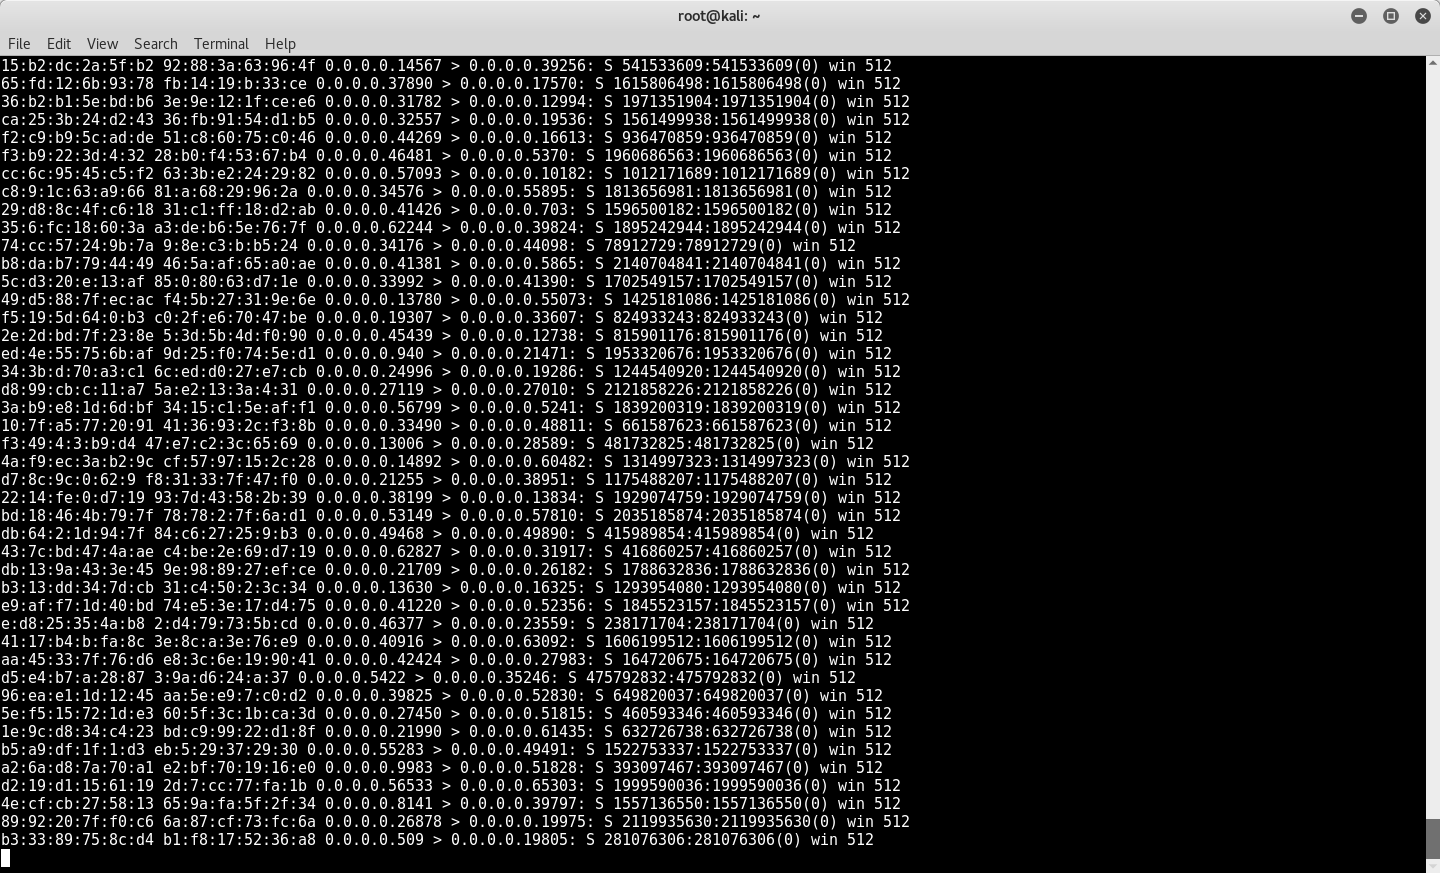
\includegraphics[width=\textwidth]{macof}
\newpage
Ako vidíme, zaplnili sme celú CAM tabuľku a switch si už nemá kam zapisovať nové vstupy.
\\
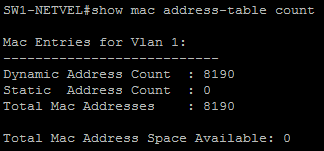
\includegraphics[width=10cm, height=8cm]{macof2}
\\
Keď si pozrieme tabuľku s MAC adresami, môžeme vidieť množstvo podhodených vstupov, ktoré prišli z portu fa0/1 od našej útočnej stanice.
\\
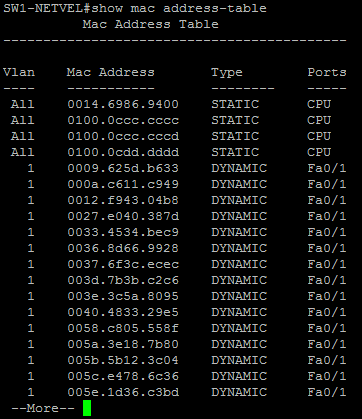
\includegraphics[width=10cm, height=8cm]{macof3}
\chapter{Zhrnutie MAC flooding útoku}
\section{Čo sa dá dosiahnuť}
Pri MAC flooding útoku dochádza k zaplneniu switcha a následne môže dôjsť k odpočúvaniu komunikácie útočníkom. V prítomnej dobe už sa to nestáva často pretože switche ktoré sa kupujú už maju zabudovanú obranu proti takýmto typom útokov. Veľmi veľa som pochopil o tomto útoku v tomto videu takže odporúčam tým ktorých to zaujíma pozrieť.\\ \url{https://www.youtube.com/watch?v=54kfAXpQtWo&ab_channel=ProfessorMesser}

%===============================================================================
